% MA211 - Lecture 09
\documentclass[pdftex, xcolor=pdftex, dvipsnames, handout]{beamer}

\usetheme{MA211}
\usepackage{thumbpdf}
\usepackage{wasysym}
%\usepackage{ucs}
\usepackage[utf8]{inputenc}
\usepackage{pgf,pgfarrows,pgfnodes,pgfautomata,pgfheaps,pgfshade}
\usepackage{verbatim}

\usepackage{eurosym}
\usepackage{euler}

\usepackage{calc}               % Simple computations with LaTeX variables
%\usepackage[hang]{caption2}     % Improved captions

\usepackage{graphicx}           % Standard graphics package

\usepackage{amsmath, amsthm, amssymb}


\newcommand{\fquad}{\mbox{\qquad}}
\newcommand{\bull}{$\bullet$ }

\newcommand {\I} {\mathcal I}
\newcommand {\calI} {\mathcal I}
\def\disint{\displaystyle\int}

\DeclareMathOperator{\D}{d}
\newcommand{\dydx}{\frac{\D y}{\D x}}

%\definecolor{gray}{rgb}{0.69, 0.69, 0.69} \newcommand{\gray}[1]{\textcolor{gray}{#1}}
\definecolor{dogreen}{rgb}{0.33, 0.42, 0.18} \newcommand{\dogreen}[1]{\textcolor{dogreen}{#1}}
\definecolor{maroon}{rgb}{.5,0.2,0.2}\newcommand{\maroon}[1]{\textcolor{maroon}{#1}}
\definecolor{greena}{rgb}{.1,0.581,0.1}\newcommand{\greena}[1]{\textcolor{greena}{#1}}

\definecolor{blue4}{rgb}{0,0,.545}
\newcommand{\Blue}[1]{\textcolor{blue}{#1}}
\newcommand{\Red}[1]{\textcolor{red}{#1}}
\definecolor{pink}{rgb}{1.,0.75,0.8}
\definecolor{darkred}{rgb}{0.5,0.0,0.0}
\definecolor{darkgreen}{rgb}{0,0.3,0.3}
\definecolor{purple}{rgb}{0,0.3,0.3}
\definecolor{darkblue}{rgb}{0.0, 0.0, .5}
\definecolor{dpurple}{rgb}{.3,.0,.3}
\newcommand{\Green}[1]{\textcolor{darkgreen}{#1}}
\newcommand{\DRed}[1]{\textcolor{darkred}{#1}}
\newcommand{\DBlue}[1]{\textcolor{darkblue}{#1}}
\newcommand{\Purple}[1]{\textcolor{dpurple}{#1}}
\newcommand{\Emph}[1]{\textcolor{darkred}{\textbf{\it #1}}}
\newcommand{\remph}[1]{\textcolor{darkred}{\textbf{\emph{#1}}}}
\newcommand{\bemph}[1]{\textcolor{darkblue}{\textbf{\emph{#1}}}}
\newcommand{\gemph}[1]{\textcolor{darkgreen}{\textbf{\emph{#1}}}}
\newcommand{\Bf}[1]{\textcolor{darkblue}{\textbf{#1}}}
\newcommand{\Gf}[1]{\textcolor{darkgreen}{\textbf{#1}}}
\newcommand{\Rf}[1]{\textcolor{red}{\textbf{#1}}}
\newcommand{\Rmf}[1]{\textcolor{red}{\mathbf{#1}}}

\newcommand{\Conj}[1]{\overline{#1}}

\newcommand{\code}[1]{\textcolor{darkblue}{\texttt{\textbf{#1}}}}
\newcommand{\icode}[1]{{\blue\texttt{\textbf{\emph{#1}}}}}
\newcommand{\gcode}[1]{{\Green{\texttt{\textbf{\emph{#1}}}}}}
\newcommand{\out}[1]{\texttt{\emph{\textbf{\Green{#1}}}}}





\newenvironment{vminipage}%
{\begin{Sbox}\begin{minipage}\begin{small}\begin{verbatim}}%
{\end{verbatim}\end{small}\end{minipage}\end{Sbox}\fbox{\TheSbox}}

\newenvironment{nminipage}%
{\begin{Sbox}\begin{minipage}}%
{\end{minipage}\end{Sbox}\fbox{\TheSbox}}


\let\Arg\relax\DeclareMathOperator{\Arg}{\mathtt{Arg}}
\let\Arg\relax\DeclareMathOperator{\e}{\mathtt{e}}

\newcommand {\AND} {\wedge}
\newcommand {\OR} {\vee}
\newcommand {\NOT} {\neg}
\newcommand {\IMPLIES} {\rightarrow}
%\newcommand {\IFF} {\leftrightarrow}
\renewcommand {\iff} {\Leftrightarrow}
\newcommand {\NAND} {\uparrow}
\newcommand {\NOR} {\downarrow}
\newcommand {\XOR} {\otimes}

\newenvironment{citemize}% Colour items
{\begin{description}}%
{\end{description}}

\newcommand {\maroonitem}{\item[\maroon{$\bullet$}]}

\newcommand {\gitem} {\item {\includegraphics[width=.4cm,angle=-10]{img/green-bullet-on-white.ps}}}
\newcommand {\ritem} {\item {\includegraphics[width=.4cm,angle=-10]{img/red-bullet-on-white.ps}}}
\newcommand {\yitem} {\item {\includegraphics[width=.4cm,angle=-10]{img/yellow-bullet-on-white.ps}}}
\newcommand {\bitem} {\item {\includegraphics[width=.4cm,angle=-10]{img/blue-bullet-on-white.ps}}}

\newcommand {\greenitem} {\item {\includegraphics[width=.4cm,angle=-10]{img/green-bullet-on-white.ps}}}
\newcommand {\reditem} {\item {\includegraphics[width=.4cm,angle=-10]{img/red-bullet-on-white.ps}}}
\newcommand {\yellowitem} {\item {\includegraphics[width=.4cm,angle=-10]{img/yellow-bullet-on-white.ps}}}
\newcommand {\blueitem} {\item {\includegraphics[width=.4cm,angle=-10]{img/blue-bullet-on-white.ps}}}

\newcommand {\eq}[1]%
  {$\DBlue{#1}$}
\newcommand {\eqd}[1]%
  {$\displaystyle\DBlue{#1}$}
%\newcommand{\eq}[1]{\boldmath \DBlue{$#1$}}


\newcommand {\csf}{\centerslidesfalse}
\newcommand {\cst}{\centerslidestrue}

\newcommand {\vecii}[2] {   \big(\begin{smallmatrix} #1 \\ #2 \end{smallmatrix}\big)}
\newcommand{\atwo}[2]{\left(\!\!\begin{array}{c} #1 \\ #2 \end{array}\!\!\right)}


\newcommand{\C}{\mathbb{C}}
\newcommand{\Q}{\mathbb{Q}}
\newcommand{\R}{\mathbb{R}}
\newcommand{\N}{\mathbb{N}}
\newcommand{\Z}{\protect\mathbb{Z}}  % protect for index.
\newcommand {\Rs}{ \mathbb{R}}
\newcommand {\Cs}{ \mathbb{C}}
\newcommand {\Rnn}{ \mathbb{R}^{n \times n}}
\newcommand {\Rn}{ \mathbb{R}^{n}}


\newcommand{\mblock}{%
\setbeamercolor*{block title}{bg=maroon,fg=white}
\setbeamercolor*{block body}{bg=white,fg=maroon}
}%

\newcommand{\bblock}{%
\setbeamercolor*{block title}{bg=Steel,fg=white}
\setbeamercolor*{block body}{bg=Mylightgray,fg=Steel}
}%

\newcommand{\gblock}{%
\setbeamercolor*{block title}{bg=Green,fg=white}
\setbeamercolor*{block body}{bg=Mylightgray,fg=darkgreen}
}%


\newcommand{\rblock}{%
\setbeamercolor*{block title}{bg=Red,fg=white}
\setbeamercolor*{block body}{bg=white,fg=Black}
}%


\newcommand{\TakeNotes}{
\includegraphics[width=2cm]{TakeNote}}

\def\eps{\varepsilon}
\newcommand {\del}[2]{ {\frac{\partial #1}{\partial #2}}}
\newcommand {\x}[1]{x^{[#1]}}
\newcommand {\delx}{ {\frac{\partial}{\partial x}}}
\newcommand {\delt}{ {\frac{\partial}{\partial t}}}
\newcommand {\dely}{ {\frac{\partial}{\partial y}}}
\newcommand {\ith}{{(i)}}
\renewcommand {\vec}[1]{ {\boldsymbol{#1}}}
\newcommand {\Oh} {\mathcal O}
\newcommand {\Err} {\mathcal E}
%\newcommand {\th} {\mathrm{th}}
\DeclareMathOperator{\fl}{fl}
\DeclareMathOperator{\sign}{sign}
\DeclareMathOperator{\Cond}{Cond} 
\DeclareMathOperator{\cond}{cond}
\DeclareMathOperator{\diag}{diag} 
\DeclareMathOperator{\sym}{sym} 
\DeclareMathOperator{\Trace}{Trace}
\DeclareMathOperator{\E}{e}

\newcommand {\Rsym}{{ \mathbb{R}^{n \times n}_\mathrm{sym}}}

\newcommand {\st} {\mathrm{st}}
\newcommand {\nd} {\mathrm{nd}}


\parskip .25cm


\theoremstyle{definition}
\newtheorem{exercise}{Exercise}[section]
\newtheorem{method}{Method}[section]

\newcommand{\Header}[1]{\begin{center}{\Large \Bf{#1}}\end{center}}

\subtitle{MA211}
\title{Lecture 9: 2nd order differential eqns }

\author{Dr Niall Madden}

\date{\Large Monday, $6^\mathrm{th}$ October  2008}


\begin{document}


\frame{

\begin{block}{}
\begin{center}
{\large \insertsubtitle}

\vspace{.1cm}

\begin{Large}
\textbf{\inserttitle}
\end{Large}

\vspace{.15cm}

% {\footnotesize \insertauthor}

\vspace{.3cm}

{ {\insertdate}}
\end{center}
\end{block}


\vspace{-0.25cm}
\begin{center}
%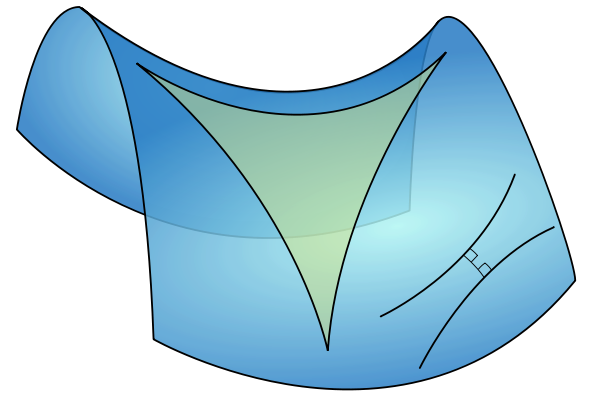
\includegraphics[height=4cm]{images/Hyperbolic}

\end{center}
}


\frame{

\Header{Class test next week...}




}

\frame{
  \frametitle{This morning}

%\begin{columns}[c]
%\column{0.5\textwidth}
%\begin{small}
 \tableofcontents
%\end{small}

%\column{0.5\textwidth}
For more details, see \Bf{17.1 } of Stewart.

%\end{columns}

}


\renewcommand{\arraystretch}{2}


\section{Recall... The Hyperbolic Functions}


\frame{


\rblock
\begin{definition}[Hyperbolic Functions]
  The \Bf{Hyperbolic cosine and sine functions} are defined as
{\Large 
\[ \cosh(x) = \frac{1}{2}\big({e^x \alert{+} e^{-x}}\big), 
\quad 
\sinh(x) = \frac{1}{2}\big({e^x \alert{\mathbf{-}} e^{-x}}\big)
\]
}
\end{definition}
\begin{center}
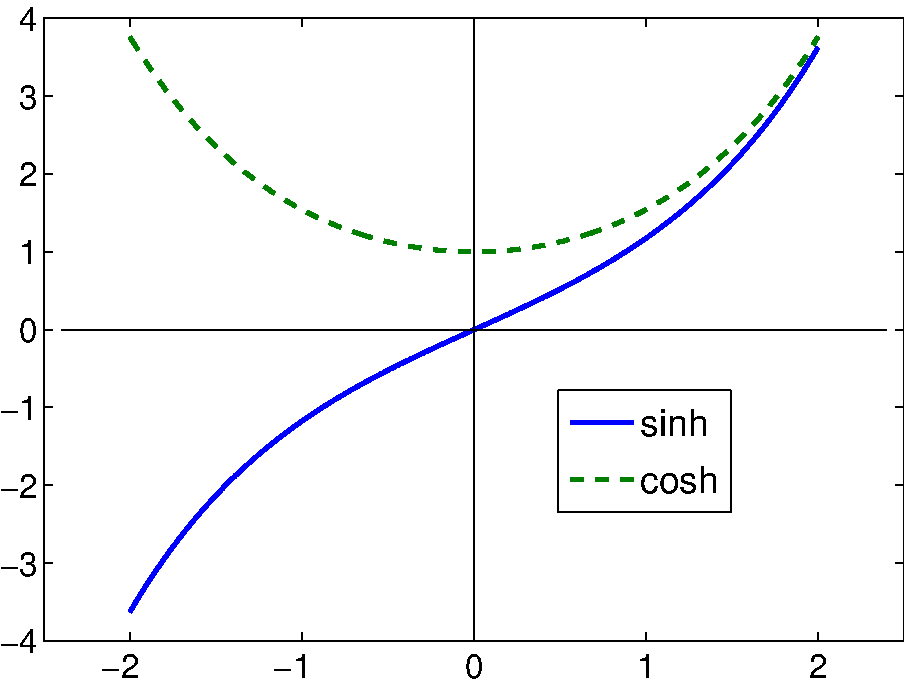
\includegraphics[width=5cm]{images/sinh}
\end{center}

}


\subsection{Properties}
\frame{

Last week we saw that:

\begin{block}{}
\begin{itemize}
\item \eqd{ \frac{d}{dx}(\sinh x) = \cosh x}

\item \eqd{ \frac{d}{dx} (\cosh x) = \sinh x}
\end{itemize}
\end{block}

}

\frame{

\begin{example}
Show that \eq{ \cosh (x+y) = \cosh x \cosh y + \sinh x \sinh y }
\end{example}
(To show this is true, we repeatedly use that \eq{e^a e^b=e^{a+b}}).\\

\vspace{3cm}

}



\subsection{Examples}

\frame{
\begin{example}[Q1 (b), Semester 1, 05/06 (v)]
 Prove that 
\[
\frac{d}{dx}\bigg( \cosh^{-1}\frac{x}{a}\bigg) = \frac{1}{\sqrt{x^2 -
    a^2}}.
\]
\end{example}
Hint:  use the Chain Rule and that  \eq{\cosh^2 y - \sinh^2y=1}.

\vspace{3cm}

}


\frame{

\begin{exercise}[Q9.1]
\begin{enumerate}[(i)]
\item Recall that \eq{\cos^2 x + \sin^2 x = 1}. 
Show that
\eq{\cosh^2 x - \sinh^2 x =1.}

\item  What are the largest possible domain for  the functions 
\eq{f(x) = \sinh(x)} and \eq{f(x) = \sinh^{-1}(x)}? Sketch their graphs.

\item Show  that \eq{\sinh(2x) = 2 \cosh(x)\sinh(x)}
\item  Prove that 
\[
\frac{d}{dx}\bigg( \sinh^{-1}\frac{x}{a}\bigg) = \frac{1}{\sqrt{a^2 + x^2}}.
\] 
\item Show that 
\[\sinh (x+y) = \sinh x \cosh y + \cosh x \sinh y.\]
\end{enumerate}
\end{exercise}

\Emph{At least one of these will appear on next Wednesday's class test}.
}




\section{More about Hyperbolic Functions}
\frame{


\begin{block}{}
The \eq{\tanh} and \eq{cotanh} functions can be defined 
\[ \tanh x = \frac{\sinh x}{\cosh x}, \qquad 
\coth x = \frac{1}{\tanh x} = \frac{\cosh x}{ \sinh x}. \]
\end{block}
\begin{center}
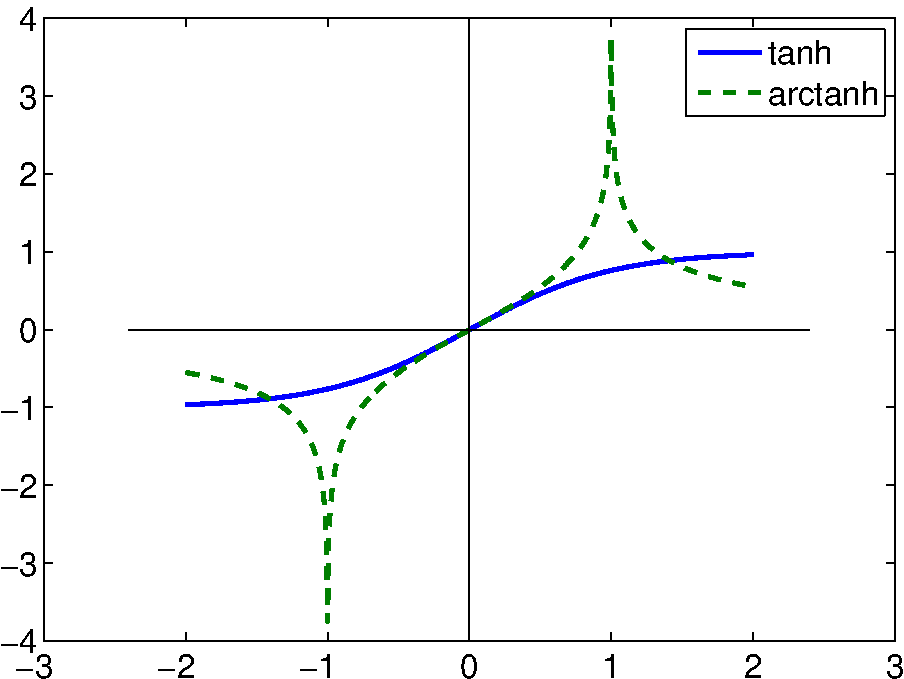
\includegraphics[width=5.6cm]{images/tanh}
\end{center}


}


\frame{

\begin{exercise}[Q9.2]
Show that
\begin{enumerate}[(i)]
\item \eq{\tanh (x) = \frac{e^{2x} - 1}{e^{2x}+1}}
\item \eq{\cosh^{-1}(x) = \ln(x + \sqrt{x^2 +1})}
\item \eqd{\frac{d}{dx} \tanh(x) = 1 - \tanh^2(x)}
\item \eqd{\frac{d}{dx} \tanh^{-1}\big(\frac{x}{a}\big) = \frac{1}{a^2 - x^2}}
\item \eqd{\cosh(2x)  = \cosh^2(x) + \sinh^2(x)}
\item \eqd{\cosh(x) + \sinh(x) = e^x}
\item \eqd{\cosh(x) - \sinh(x) = e^{-x}}
\end{enumerate}
\end{exercise}
}


%\frame{
%\begin{example}
% Differentiate $\tanh x$.
%\end{example}
%\Bf{Solution:}
%}


\section{Differential Equations}

\frame{
Now that we have the exponential, logarithmic, trigonometric and
hyperbolic functions at our disposal, we can solve some differential
equations.


The DEs that we'll look at now are of 
\Header{2nd Order, Constant Coefficient, Homogeneous type.}

\begin{example}
\[\frac{d^2y}{dx^2} + \frac{dy}{dx} - 2y = 0 \Longleftrightarrow 
y''(x) + y'(x) -2y(x) =0.\]
\end{example}

}



\frame{

\Header{2nd Order, Constant Coefficient, Homogeneous type.}

\begin{block}{}
\[ a \frac{d^2y}{dx^2} + b \frac{dy}{dx} + cy = 0 \Longleftrightarrow 
a y''(x) + by'(x) + cy(x) =0.\]
where \eq{a}, \eq{b} and \eq{c} are constants (real numbers).
\end{block}

\pause We will see that all the solutions to these equations come in
one of the following forms:
\begin{enumerate}
\item \eqd{A e^{R_1x} + B e^{R_2x}},

\item \eqd{(A e + B  x) e^{Rx}}.

\item \eqd{e^{k x}\big(A \cos(\omega t) + B \sin(\omega t)\big)}

\end{enumerate}
where \eq{A} and \eq{B} are arbitrary constants.


}

\frame{
To solve these equations we will:
\begin{itemize}
\item First assume that the solution is \eq{y = C e^{Rx}}.
\item Substitute this into the DE to get a quadratic equation for
  \eq{R}.
\item Call the two solutions to this equation \eq{R_1} and \eq{R_2}.

\item Where its useful, we'll express the solutions in terms of trig
  functions using \Bf{Euler's Formula}:
\begin{block}{}
\[  e^{ix}  = \cos(x) + i \sin(x) \qquad \text{ where } i = \sqrt{-1}\]
\end{block}
%or using Hyperbolic functions:a
%\begin{block}{}
%\[
% \cosh(x) = \frac{1}{2}\big(e^x + e^{-x}\big), 
%~ \text{ and }  ~ 
% \sinh(x) = \frac{1}{2}\big(e^x - e^{-x}\big). 
%\]
%\end{block}
\end{itemize}
}


\section{Linear Combinations of Solutions}
\frame{

\begin{block}{}
Suppose that \eq{y} is a solution to the differential equation
\[
a y'' + by' + cy =0,
\]
Then so too is \eq{\alert{K}y} for any constant \eq{\alert{K}}
\end{block}


\vspace{3cm}


}

\frame{
\begin{block}{}
If \eq{y_1} and \eq{y_2} are both solutions to 
\[
a y''(x) + by'(x) + cy(x) =0,
\]
The so too is any function \eq{y(x) = A y_1(x) + B y_2(x)}.
\end{block}

\vspace{3cm}

}

\frame{


\begin{example}{}
Find \eq{r} such that \eqd{y(x) = e^{Rx}} is a  solution to the equation:
\[
y'' + 5 y' + 4y =0.
\]
\end{example}

\vspace{4cm}

}

\section{The Axillary Equation}
\frame{

In the previous example, the key part is solving the quadratic equation
\[ aR^2 + bR + c=0.\]
\[ R = \frac{-b \pm \sqrt{b^2 -4ac}}{2a}. \]
This is called \Bf{The Auxiliary Equation}.

Also, \eq{D=b^2 -4ac} is called the \Bf{Discriminant}.

\pause
\begin{itemize}
\item If \eq{D>0}, then there are two real-valued solutions to the
  auxiliary equation.
\item If \eq{D=0}, then the auxiliary equation has only one solution.
\item If \eq{D<0}, the solutions to the auxiliary equation are
  \Emph{complex valued}.
\end{itemize}


}

\section{$D>0$}
\rblock
\frame{

The easiest case is \eq{D=b^2 -4ac>0}.
\begin{block}{$D>0$}
If \eq{D=b^2 -4ac>0}, then the auxiliary equation
\[ ar^2 + br + c=0\]
has two solutions:
\[
R_1 = \frac{-b + \sqrt{b^2 -4ac}}{2a}, \qquad
R_2 = \frac{-b - \sqrt{b^2 -4ac}}{2a}, 
\]
and the general solution is
\[
y (x) = A e^{R_1x} + B e^{R_2x}.
\]
\end{block}

}

\gblock
\frame{
\begin{example}
Write down the general solution to the differential equation
\[
y'' - 2y' - 3 y=0.
\]
Verify your answer is correct.
\end{example}
\Bf{Solution:}

\vspace{4cm}

}

\end{document}
\bblock
\frame{
\begin{example}
Find the  general solution to the differential equation
\[
y'' - 4 y=0.
\]
and express the solution in terms of \eq{\sinh} and \eq{\cosh}

\end{example}
\Bf{Solution:}

\vspace{4cm}

}

\rblock
\section{$D=0$}
\frame{
The next easiest case is \eq{D=b^2 -4ac=0}.
\begin{block}{$D=0$}
If \eq{D=b^2 -4ac=0}, then the auxiliary equation
\[ ar^2 + br + c=0\]
has just one  solution:
\[
R = \frac{-b}{2a}, \qquad
\]
and the general solution is
{\Large \[
{ y (x) = A e^{Rx} + B \alert{x} e^{Rx}.}
\]}
\end{block}

}

\frame{
\begin{example}
Find the general solution to the equation
\[
y'' + 2y' + y=0,
\]
and verify your solution.
\end{example}
\Bf{Solution:}

\vspace{4cm}
}

\frame{
\bblock
\begin{exercise}
Find the general solution to the equation
\[
\frac{3}{4}y'' + 3y' + 3y=0.
\]
\end{exercise}
}

\frame{
\bblock
\begin{example}

Suppose the coefficients of the differential equation
\[
a y'' + by' + cy=0.
\]
are such that  \eq{b^2=4ac}. If  \eqd{y_1=e^{rx}} is a solution, where
\eqd{r=-b/2a}, then show that \eqd{y_2 = xe^{rx}}  is also
a solution. 

\end{example}

\vspace{3cm}

}


\end{document}
